\chapter{ideal Fermi systems}
\begin{itemize}
	\item $f_n(z)$ 是 Fermi-Dirac function,
	\begin{equation}
		f_n(z) \equiv \frac{1}{\Gamma(n)} \int_0^\infty \frac{x^{n - 1}}{z^{- 1} e^x + 1} dx = z - \frac{z^2}{2^n} + \frac{z^3}{3^n} - \cdots, \quad \text{and} \quad f_n'(z) = \frac{1}{z} f_{n - 1}(z),
	\end{equation}
	是单调递增函数 (当 $n > 0$), $- 1 < z < 1$, 且 $f_n(1) = (1 - 2^{1 - n}) \zeta(n)$.
	\begin{itemize}
		\item 与 Bose-Einstein statistics 不同, $f_n(z)$ 在 $z = 1$ 没有极点, 只是它的级数展开在 $z > 1$ 发散 (因为 $z = - 1$ 处有极点).
		
		\item $g_n(z) = - f_n(- z) = \mathrm{Li}_n(z)$, 称为 \href{https://en.wikipedia.org/wiki/Polylogarithm}{Polylogarithm}, 见下图:
		
		\begin{figure}[H]
			\centering
			\includegraphics[scale=0.5]{figures/plot of Li_n(z) with n=frac{3}{2}.pdf}
			\caption{plot of $\mathrm{Li}_n(z)$ with $n=\frac{3}{2}$.}
		\end{figure}
	\end{itemize}
\end{itemize}

\section{thermodynamic behavior of an ideal Fermi gas}
\begin{itemize}
	\item ideal Fermi gas 的 grand partition function 为
	\begin{equation}
		\frac{P V}{k_B T} = \ln Z_\text{GC} = N_s \Big( \frac{V}{\lambda^3} f_{5 / 2}(z) + \underbrace{\ln(1 + z)}_{\text{always negligible}} \Big),
	\end{equation}
	对 $\mu$ 的取值范围没有限制.
	
	\begin{tcolorbox}[title=calculation:]
		粒子能量的简并度见 \eqref{7.1.2}, 所以
		\begin{equation}
			\ln Z_\text{GC} = N_s \ln(1 + z) + \int_0^\infty \ln(1 + z e^{- \beta \epsilon}) g(\epsilon) d\epsilon = \cdots,
		\end{equation}
		且
		\begin{equation}
			N_0 = \frac{N_s}{z^{- 1} + 1} < N_s \Longrightarrow \ln(1 + z) = - \ln(1 - N_0 / N_s) \sim N_0 / N_s \ll N.
		\end{equation}
	\end{tcolorbox}
	
	\item 得到
	\begin{equation}
		\begin{dcases}
			N = N_s \frac{V}{\lambda^3} f_{3 / 2}(z) \\
			U = \frac{3}{2} N_s k_B T \frac{V}{\lambda^3} f_{5 / 2}(z) \\
			S = N k_B \Big( \frac{5}{2} \frac{f_{5 / 2}(z)}{f_{3 / 2}(z)} - \ln z \Big) \\
			\frac{C_V}{N k_B} = \frac{15}{4} \frac{f_{5 / 2}(z)}{f_{3 / 2}(z)} - \frac{9}{4} \frac{f_{3 / 2}(z)}{f_{1 / 2}(z)}
		\end{dcases},
	\end{equation}
	注意到 $U = \frac{3}{2} P V$ 依然成立.
	
	\item 经典极限 $n \lambda^3 \ll 1$ 对应 $z \ll 1$, 此时 $f_n(z) \simeq z$, 代入可以得到理想气体的各热力学量.
	
	\item 对 equation of state 作 virial expansion,
	\begin{equation}
		\begin{dcases}
			\frac{P V}{N k_B T} = \sum_{l = 1}^\infty (- 1)^{l - 1} a_l (n \lambda^3 / N_s)^{l - 1} \\
			\frac{C_V}{N k_B} = \frac{3}{2} \sum_{l = 1}^\infty (- 1)^{l - 1} \frac{5 - 3 l}{2} a_l (n \lambda^3 / N_s)^{l - 1}
		\end{dcases},
	\end{equation}
	其中系数 $a_l$ 见 \eqref{7.1.8}, 展开适用于 $n \lambda^3 / N_s \ll 1$.
\end{itemize}

\subsection{degenerate ideal Fermi gas}
\subsubsection{ground state of the system: $T \rightarrow 0$}
\begin{itemize}
	\item 当 $n \lambda / N_s \rightarrow \infty, z \rightarrow \infty$ 时 ($T \rightarrow 0$), mean occupation number 变成 step function,
	\begin{equation}
		\braket{n_i} = \begin{dcases}
			g_i & \epsilon < \mu_0 \\
			0 & \epsilon > \mu_0
		\end{dcases},
	\end{equation}
	其中 $\mu_0 \equiv \epsilon_F \equiv \frac{p_F^2}{2 m}$ 称为 Fermi energy, $p_F$ 称为 Fermi momentum, $k_B T_F \equiv \epsilon_F$ 称为 Fermi temperature,
	\begin{equation}
		\epsilon_F \equiv k_B T_F = \Big( 6 \pi^2 n / N_s \Big)^{\frac{2}{3}} \frac{\hbar^2}{2 m}, \quad p_F = \Big( 6 \pi^2 n / N_s \Big)^{\frac{1}{3}} \hbar.
	\end{equation}
	
	\begin{tcolorbox}[title=calculation:]
		\begin{equation}
			N = \int_0^{\mu_0} g(\epsilon) d\epsilon = N_s 2 \pi \frac{V / \lambda^3}{(\pi k_B T)^{3 / 2}} \frac{2}{3} \mu_0^{3 / 2} \Longrightarrow \mu_0 = \Big( \frac{3}{4 \pi} n \lambda^3 / N_s \Big)^{\frac{2}{3}} \pi k_B T = \cdots
		\end{equation}
	\end{tcolorbox}
	
	\item 此时, Fermi gas 处于能量基态,
	\begin{equation}
		\frac{E_0}{V} = \frac{3}{2} P_0 = N_s \frac{2 \pi}{5 m h^3} \underline{p_F^5} = \frac{3}{5} n \epsilon_F = \frac{3}{5} \Big( 6 \pi^2 / N_s \Big)^{\frac{2}{3}} \frac{\hbar^2}{2 m} \underline{n^{5 / 3}},
	\end{equation}
	可见 $P_0 \propto n^{5 / 3}$.
\end{itemize}

\subsubsection{with finite temperature}
\begin{itemize}
	\item 将 Fermi-Dirac function 关于 $\ln z = \beta \mu$ 展开, 得到
	\begin{equation} \label{8.1.10}
		\begin{dcases}
			N = N_s \frac{4 \pi}{3} V \Big( \frac{2 m}{h^2} \beta \ln z \Big)^{\frac{3}{2}} \Big( 1 + \frac{\pi^2}{8} (\ln z)^{- 2} + \cdots \Big) \Longrightarrow \mu \simeq \epsilon_F \Big( 1 - \frac{\pi^2}{12} (\beta \epsilon_F)^{- 2} \Big) \\
			U = \frac{3}{2} P V = \frac{3}{5} N \epsilon_F \Big( 1 + \frac{5 \pi^2}{12} (\beta \epsilon_F)^{- 2} + \cdots \Big) \\
			\frac{C_V}{N k_B} = \frac{\pi^2}{2} \frac{1}{\beta \epsilon_F} + \cdots \\
			S = N k_B \Big( \frac{\pi^2}{2} (\beta \epsilon_F)^{- 2} + 
			\cdots \Big)
		\end{dcases},
	\end{equation}
	可见 $T \rightarrow 0$ 时 $S \rightarrow 0$, 符合预期.
	
	\item ideal Fermi gas 的 specific heat 如下图所示:
	
	\begin{figure}[H]
		\centering
		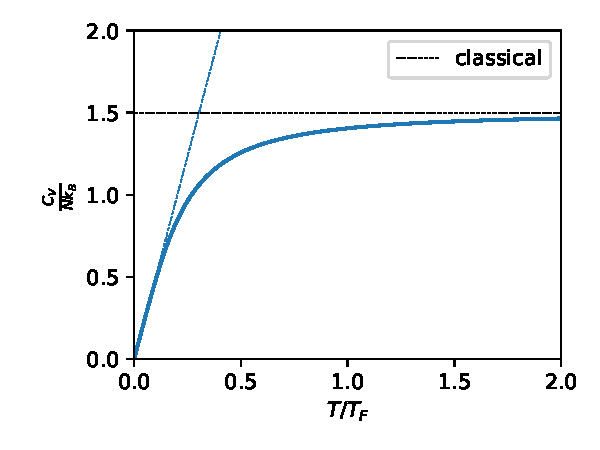
\includegraphics[scale=0.8]{figures/specific heat of an ideal Fermi gas.pdf}
		\caption{specific heat of an ideal Fermi gas.}
	\end{figure}
\end{itemize}

\section{magnetic behavior of an ideal Fermi gas}
\begin{itemize}
	\item Maxwell-Boltzmann statistics 给出的结果见 section \ref{3.7}.
\end{itemize}

\subsection{Pauli paramagnetism}
\begin{itemize}
	\item Pauli 将 alkali metal 中的 conducting electrons 视为 highly degenerate Fermi gas.
	
	\item 电子的 Hamiltonian 为
	\begin{equation}
		H = \frac{|\vec{p}|^2}{2 m} - \mu_0 \vec{\mu}^* \cdot \vec{H},
	\end{equation}
	其中 $\vec{\mu}^* = - \mu_B \vec{\sigma}$ (见 \eqref{5.3.1}). 因此, 系统的 grand partition function 为
	\begin{equation}
		\ln Z_\text{GC} = \frac{V}{\lambda^3} \Big( f_{5 / 2}(z e^{- \beta \epsilon_{M, +}}) + f_{5 / 2}(z e^{- \beta \epsilon_{M, -}}) \Big).
	\end{equation}
	
	\begin{tcolorbox}[title=calculation:]
		将电子的能量分成 $\epsilon = \epsilon_K + \epsilon_M$, 其中 $\epsilon_M = \pm \mu_0 \mu_B H$, 所以
		\begin{align}
			\ln Z_\text{GC} &= \sum_{\epsilon_K, \epsilon_M} g_K(\epsilon_K) \ln(1 + z e^{- \beta (\epsilon_K + \epsilon_M)}) \notag \\
			&= \frac{V}{\lambda^3} \Big( f_{5 / 2}(z e^{- \beta \epsilon_{M, +}}) + f_{5 / 2}(z e^{- \beta \epsilon_{M, -}}) \Big).
		\end{align}
	\end{tcolorbox}
	
	\item 得到
	\begin{equation} \label{8.2.4}
		N_{\pm} = - \frac{1}{\beta} \frac{\partial}{\partial \epsilon_{M, \pm}} \ln Z_\text{GC} = \frac{V}{\lambda^3} f_{3 / 2}(z e^{- \beta \epsilon_{M, \pm}}) \simeq \frac{V}{6 \pi^2} \Big( \frac{2 m}{\hbar^2} (\epsilon_F - \epsilon_{M, \pm}) \Big)^{\frac{3}{2}},
	\end{equation}
	因此
	\begin{align}
		V \braket{M_z} &= N \braket{\mu^*_z} = N_+ (- \mu_B) + N_- (+ \mu_B) \notag \\
		&\simeq \frac{4 \pi^2 V \mu_B}{3} \Big( \Big( \frac{2 m}{h^2} (\epsilon_F + \mu_0 \mu_B H) \Big)^{\frac{3}{2}} - \Big( \frac{2 m}{h^2} (\epsilon_F - \mu_0 \mu_B H) \Big)^{\frac{3}{2}} \Big),
	\end{align}
	系统的 low-field magnetic susceptibility is
	\begin{equation}
		\chi_0 = \lim_{H \rightarrow 0} \frac{M_z}{H} = 4 \pi \mu_0 \mu_B^2 \Big( \frac{2 m}{h^2} \Big)^{\frac{3}{2}} \epsilon_F^{1 / 2} = \frac{3}{2} \frac{N}{V} \frac{\mu_0 \mu_B^2}{\epsilon_F}, \quad \epsilon_F(n, H = 0) = \frac{h^2}{2 m} \Big( \frac{3 N}{8 \pi V} \Big)^{\frac{2}{3}},
	\end{equation}
	其中, 用 \eqref{8.2.4} 得到 $\epsilon_F$ 的表达式, 下标 $0$ 表示 $T \rightarrow 0$ (again, highly degenerate).
	
	\begin{itemize}
		\item 对比高温极限 \eqref{3.7.18} ($g = 2, j = \frac{1}{2}$),
		\begin{equation} \label{8.2.7}
			\chi_\infty = \frac{N}{V} \frac{\mu_0 \mu_B^2}{k_B T}.
		\end{equation}
	\end{itemize}
	
	\noindent\rule[0.5ex]{\linewidth}{0.5pt} % horizontal line
	
	\item 有限温度下,
	\begin{align}
		V \braket{M_z} &= N_+ (- \mu_B) + N_- (+ \mu_B) \overset{H \rightarrow 0}{=} \Big( \frac{V}{\lambda^3} f'_{3 / 2}(z) 2 z \beta \mu_0 \mu_B H \Big) \mu_B \notag \\
		&= 2 \frac{V}{\lambda^3} f_{1 / 2}(z) \frac{\mu_0 \mu_B^2}{k_B T} H = N \frac{f_{1 / 2}(z)}{f_{3 / 2}(z)} \frac{\mu_0 \mu_B^2}{k_B T} H.
	\end{align}
	\begin{itemize}
		\item 在有限 (但依然简并, $T \ll T_c$) 温度下, 参考 \eqref{8.1.10},
		\begin{equation}
			V \braket{M_z} \overset{H \rightarrow 0}{=} \Big( 2 \frac{V}{\lambda^3} f_{1 / 2}(z) \beta \mu_0 \mu_B H \Big) \mu_B \simeq V \braket{M_z}_{T = 0} \Big( 1 - \frac{\pi^2}{12} \frac{1}{(\beta \epsilon_F)^2} \Big),
		\end{equation}
		因此
		\begin{equation}
			\chi \overset{T \ll T_F}{\simeq} \chi_0 \Big( 1 - \frac{\pi^2}{12} \frac{1}{(\beta \epsilon_F)^2} \Big).
		\end{equation}
		
		\item 高温极限下, $z \ll 1 \Longrightarrow f_n(z) \simeq z - \frac{z^2}{2^n}$,
		\begin{align}
			& V \braket{M_z} \simeq \chi_\infty \Big( 1 - \Big( \frac{1}{2^{1 / 2}} - \frac{1}{2^{3 / 2}} \Big) z \Big) H \simeq \chi_\infty \Big( 1 - \frac{1}{2^{5 / 2}} n \lambda^3 \Big) H \notag \\
			\Longrightarrow & \chi \overset{T \gg T_F}{\simeq} \chi_\infty \Big( 1 - \frac{1}{2^{5 / 2}} n \lambda^3 \Big).
		\end{align}
	\end{itemize}
\end{itemize}

\subsection{Landau diamagnetism}
\begin{itemize}
	\item 单个电子的 Hamiltonian, 及其能级和能级简并度 $g(\epsilon)$ 见 appendix \ref{A}.
	
	\item 系统的 grand partition function 为
	\begin{equation}
		\ln Z_\text{GC} = V \frac{B e}{h^2} \sqrt{2 \pi m k_B T} \sum_{j = 0}^\infty f_{3 / 2}(z e^{- \beta 2 \hbar \omega_L (j + \frac{1}{2})}).
	\end{equation}
	
	\begin{tcolorbox}[title=calculation:]
		\begin{align}
			\ln Z_\text{GC} &= L_x L_y \frac{B e}{h} \sum_{j, n_z = 0}^\infty \ln \Big( 1 + z e^{- \beta (2 \hbar \omega_L (j + \frac{1}{2}) + \frac{h^2}{8 m L_z^2} n_z^2)} \Big) \notag \\
			&\simeq L_x L_y \frac{B e}{h} \sum_{j = 0}^\infty \int_{- \infty}^\infty \frac{L_z dp_z}{h} \ln \Big( 1 + z e^{- \beta (2 \hbar \omega_L (j + \frac{1}{2}) + \frac{p_z^2}{2 m})} \Big) \notag \\
			&= V \frac{B e}{h^2} \sqrt{2 m k_B T} \sum_{j = 0}^\infty \int_0^\infty \ln \Big( 1 + z e^{- \beta 2 \hbar \omega_L (j + \frac{1}{2})} e^{- x} \Big) x^{- 1 / 2} dx,
		\end{align}
		令 $z_j = z e^{- \beta 2 \hbar \omega_L (j + \frac{1}{2})}$, 积分部分为
		\begin{equation}
			I(z_j) = 2 \int_0^\infty \frac{x^{1 / 2}}{z_j^{- 1} e^{x} + 1} dx = \sqrt{\pi} f_{3 / 2}(z_j).
		\end{equation}
	\end{tcolorbox}
\end{itemize}

\subsubsection{at high temperature}
\begin{itemize}
	\item 高温极限下 $z \ll 1$, 系统的 partition function 化为
	\begin{equation}
		\ln Z_\text{ZG} \simeq V \frac{B e}{h^2} \sqrt{2 \pi m k_B T} \sum_{j = 0}^\infty z e^{- \beta 2 \hbar \omega_L (j + \frac{1}{2})} = V \frac{B e}{h^2} \sqrt{2 \pi m k_B T} z \Big( 2 \sinh \beta \hbar \omega_L \Big)^{- 1}.
	\end{equation}
	
	\item 得到
	\begin{equation}
		\begin{dcases}
			N = \frac{z V}{\lambda^3} \frac{x}{\sinh x} \\
			V M = - \frac{\partial U}{\partial B} = \frac{1}{\beta} \frac{\partial}{\partial B} \ln Z_\text{GC}(T, V, z) = - N \mu_\text{eff} \Big( \coth x - \frac{1}{x} \Big)
		\end{dcases},
	\end{equation}
	其中 $x = \beta \hbar \omega_L = \beta \mu_\text{eff} B$,
	\begin{equation}
		\mu_\text{eff} = \frac{e \hbar}{2 m}.
	\end{equation}
	\begin{itemize}
		\item 结果类似于 Langevin paramagnetism, 见 section \ref{3.7}, 但负号是 quantization 的结果.
	\end{itemize}
	
	\item 注意到 $\mu_\text{eff} B \ll k_B T \Longrightarrow B \approx \mu_0 H$, 得到
	\begin{equation}
		\chi_\infty \simeq - \frac{N}{V} \frac{\mu_0 \mu_\text{eff}^2}{3 k_B T},
	\end{equation}
	结合 \eqref{8.2.7}, 高温下 electron gas 的 susceptibility 为
	\begin{equation}
		\boxed{\chi_\infty = \frac{N}{V} \frac{\mu_0}{k_B T} \Big( \mu_B^2 - \frac{1}{3} \Big( \frac{e \hbar}{2 m} \Big)^2 \Big)}.
	\end{equation}
\end{itemize}

\subsubsection{at all temperature with weak magnetic field}
\begin{itemize}
	\item 不再要求 $z$ 是小量, 但依然有 $\mu_0 \mu_\text{eff} H \approx \mu_\text{eff} B \ll k_B T$.
	
	\item ...
\end{itemize}

\section{the electron gas in metals}

\section{ultracold atomic Fermi gases}

\section{statistical equilibrium of white dwarf stars}
